\subsection{Datenstrukturen und Algorithmen}
\subsubsection{Ringbuffer}

\begin{wrapfigure}{r}{0.45\textwidth}
    % \begin{figure}[h]
     \vspace{-\baselineskip}
         \centering
         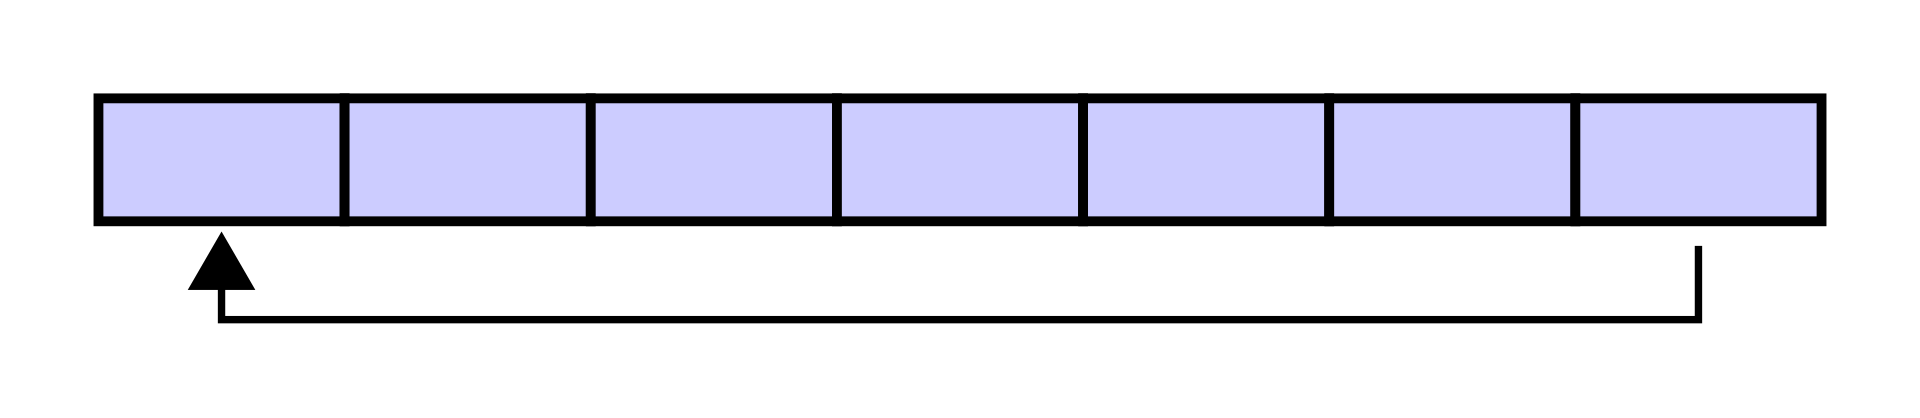
\includegraphics[scale=0.1]{Pictures/circular_buffer.png}
         \caption{\textit{Ringbuffer \citep{ImgBuffer}}}
         \label{img:Ringbuffer}
    % \end{figure}
 \end{wrapfigure}

Der Ringbuffer ist eine Datenstruktur, die nach dem \ac{FIFO}-Prinzip arbeitet. Dies bedeutet, dass die Daten, welche
zuerst in den Buffer geschrieben wurden, auch zuerst wieder ausgelesen werden. 

\smallskip

Die zu schreibenden Daten werden in ein Array von bestimmter Länge N geschrieben. Läuft das Array voll, werden die neuen Zeichen
wieder an den Anfang geschrieben. Zur Orientierung werden zwei Zähler eingeführt, der Lese- und Schreibindex. Der Leseindex
zeigt die aktuelle Position im Array an. Der Schreibindex zeigt, bis an welche Stelle
neue Daten geschrieben wurden.  

Haben Lese- und Schreibindex den selben Wert, gilt der Buffer als leer. 

\smallskip

Wird ein Zeichen in den Ringbuffer geschrieben, wird der Schreibindex inkrementiert. Sobald ein Zeichen gelesen wird, wird der Leseindex
inkrementiert. Erreichen die beiden Indizes das Ende des Arrays, werden sie auf 0 zurückgesetzt.


\subsubsection{Cyclic Redundancy Check}
\label{subsub: CRC16}

Cyclic Redundancy Check (\textit{deutsch Zyklische Redundanzprüfung}), kurz \textbf{CRC}, ist eine Methode zur Erkennung von Fehlern bei 
der Übertragung. Es ist nur möglich, zufällige Fehler zu erkennen, wie sie z.B. durch Übertragungsfehler oder Rauschen auf der Leitung entstehen \citep{IK_VL}.

\smallskip

Den zu übertragenden Daten wird ein zuvor berechneter Wert angehängt. Mittels dieses Wertes kann die Empfängerseite feststellen, ob die Daten korrekt 
übertragen wurden oder ob ein Fehler vorliegt. 

\smallskip

CRC nutzt zur Überprüfung der Daten die Polynomdivsion. Die zu übertragenden Daten werden als Polynom dargestellt.

\smallskip

Die Bitfolge \begin{math}
    10101010
\end{math}  entspricht dem Polynom \begin{math}
    1*x^7+0*x^6+1*x^5+0*x^4+1*x^3+0*x^2+1*x+0
\end{math}.
Das Polynom der Bitfolge wird durch ein zuvor festgelegtes CRC-Polynom geteilt. Der Rest dieser mathematischen Operation repräsentiert den CRC-Wert. Dieser Wert
wird anschließend bei der Datenübertragung an die zu übertragende Nachricht angehängt.

\smallskip

Empfängerseitig wird nun abermals eine Polynomdivision durchgeführt. Ist das Ergebnis der Polynomdivision empfangene Nachricht inkl. CRC-Wert dividiert durch das
CRC-Polynom gleich 0, wurde die Nachricht korrekt übertragen \citep{IK_VL}.


\subsection{STM32 Hardware Abstraction Layer und CubeMX}

Der \ac{HAL} ist eine Schnittstelle zwischen der untersten Firmwareschicht des STM32 und der Software, welche der Nutzer schreibt. Durch die Benutzung des
\acp{HAL} müssen keine einzelnen Register mittels Assembler gesetzt werden. Die Konfiguration wird dadurch stark vereinfacht und die Fehleranfälligkeit verringert.

\smallskip

Die dazu notwendigen Libraries werden vom Hersteller (ST) bereitgestellt und dokumentiert \citep{HAL_Description}. 

\smallskip

Funktionen, welche durch den \ac{HAL} bereitgestellt werden, sind zu erkennen an einem vorgestellten \textit{HAL}. Folgende Funktion schaltet z.B. einen \ac{GPIO} um:

\smallskip

\begin{lstlisting}[caption={\textit{Umschalten von \acs{GPIO}}}]
   void HAL_GPIO_TogglePin(GPIOx, GPIO_Pin);
\end{lstlisting}

\smallskip

Neben dem \ac{HAL} stellt der Hersteller ein weiteres Tool zur Verfügung (Cube MX \citep{CubeMX}), welches die schnelle Erstellung des Initialiserungscodes 
für die Peripherie und sonstige Funktionen ermöglicht. Dies verringert ebenfalls die Fehleranfälligkeit und vereinfacht die Programmierung.

\smallskip

Mittels einer graphischen Oberfläche können den verschieden Anschlüssen des \ac{uC} Funktionen zugewiesen (z.B. \acs{I2C}) und Taktfrequenzen
konfiguriert werden.

\vspace{0.5cm}

\begin{figure}[h]
    \vspace{-\baselineskip}
        \centering
        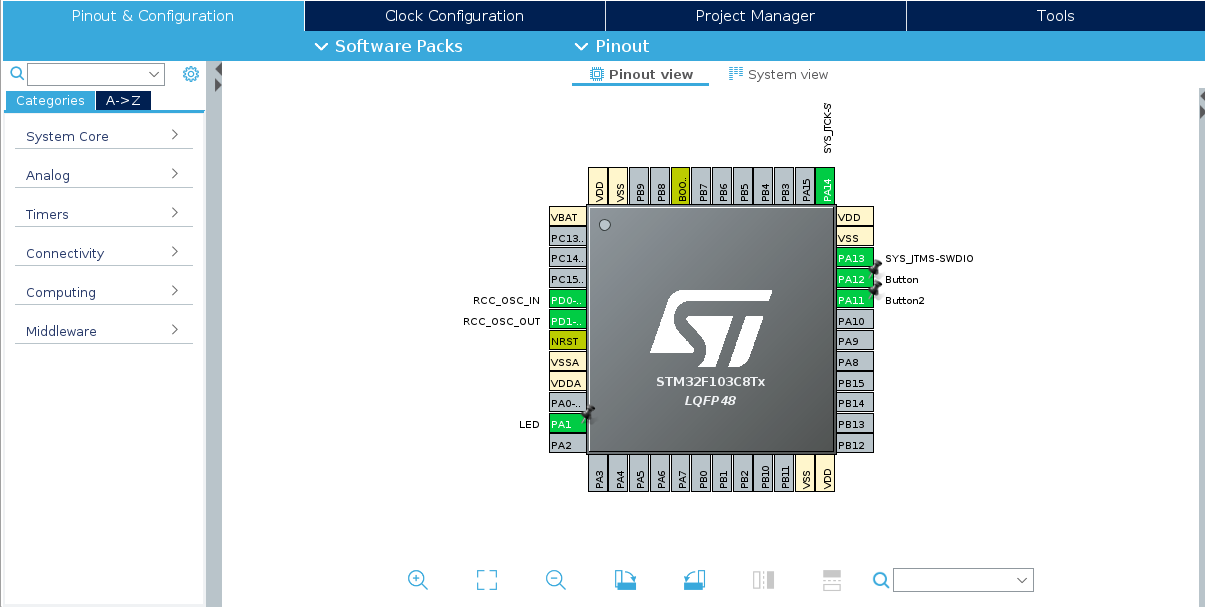
\includegraphics[scale=0.3]{Pictures/cubeMX.png}
        \caption{\textit{CubeMX}}
        \label{img:CubeMX}
\end{figure}